\documentclass[UTF8]{ctexart}
    \title{\huge Code Reading Report V2}
    \author{\large 2015011308 唐适之}
    \date{}
    \usepackage[top=1in, bottom=1in, left=1.25in, right=1.25in]{geometry}
    \usepackage{enumitem}
	\usepackage{graphicx}
	\usepackage{amsmath}
	\usepackage{amssymb}
	\usepackage[amsmath,thref,thmmarks]{ntheorem}
    \renewcommand{\figurename}{Figure}

\begin{document}
    
    \maketitle

    \section{Introduction}

        \subsection{Purpose of the Report}

            This report describes the architecture and system design of \textit{LiquidFun}, including its components, workflow, advanced techniques, and key design principles. This is not a API reference, and will not cover all the detailed functions.

        \subsection{Scope of the Project}

            \textit{LiquidFun} is a 2D rigid-body and fluid simulation C++ library for games based upon \textit{Box2D}. It provides support for procedural animation of physical bodies to make objects move and interact in realistic ways\footnote{http://google.github.io/liquidfun/ Overview}. It brings particles to \textit{Box2D} so as to simulate fluid. \textit{LiquidFun} is not a physical simulator for scientific analysing. It provides an approximate but efficient way of calculation. \textit{LiquidFun} is either not a game framework. It only provides an interface to calculate the physics, but does not involves in displaying and controling.

        \subsection{Reference Material}

            \begin{itemize}
                \item \textit{LiquidFun Programmer's Guide}.

                      http://google.github.io/liquidfun/Programmers-Guide/html/index.html
                      
                \item \textit{LiquidFun API Documentation}.

                      http://google.github.io/liquidfun/API-Ref/html/index.html
            \end{itemize}

    \section{System Overview}

        \subsection{Architectural Design}
            
            There are three major modules inherited from \textit{Box2D}: Common, Collision and Dynamics. The Common module is an infrastructure, which provides memory allocation, math, settings and data structures. The Collision module takes charge of static geometry, which defines shapes and handles geometric queries. The Dynamics module simulates the physics using the two module above.

            The Dynamics module can only do with rigid bodies, and therefore a Particle moudle is added in \textit{LiquidFun}, which provides simulation of particles. There is also a Rope module which seems to be uncompleted however.

            The figure below is the relations among these modles, extended from the graph in \textit{Box2D} document, which describes the three \textit{Box2D} modules. In this figure, the modules below make use of the modules above.

            \begin{figure}[ht]
                \centering
                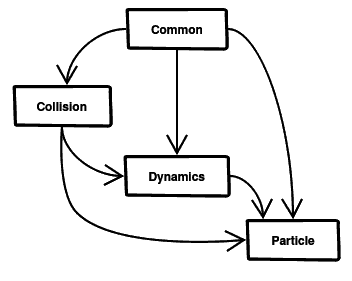
\includegraphics[width=.5\textwidth]{modules.png}
                \caption{Modules}
            \end{figure}

\end{document}

